\documentclass[main.tex]{subfiles}
\begin{document}
\part{Mechanics}


Material from this chapter mainly comes from NCSU's PY411 and PY412 classical
mechanics courses. In addition to the provided material, the course covered perturbation
theory and nonlinear dynamics/chaos; I hope to instead contain these in notes on math
and special topics, respectively.

Note that this section does not take relativistic effects into consideration, so definitions
such as those of momentum and energy may differ from the relativistic definitions.

\chapter{Fundamental Principles}

We begin with the basic fundamental principles of physics. These largely begin with
Newton's laws and apply to a single particle.

\section{Newton's Laws}


Newton's laws are where the basic principles of physics begin. They are as follows:

\begin{enumerate}
\item An object in motion will stay in motion
\item Force produces an acceleration proportional to mass
\item Each action has an equal and opposite reaction
\end{enumerate}

It is important to realize that Newton's laws require an inertial reference frame, that is,
a frame that is moving with constant velocity without any acceleration. Velocity and
acceleration with respect to what? Space itself -- Newton's concept of space was absolute.

The first law, also referred to as the Law of Inertia, states that in the absence of forces,
a particle will continue moving at a constant velocity.

The second law, often described in the mathematical form of \cref{eqn: newton-second},
is one of the core equations used in physics. In a sense, it defines mass as a quantity
that resists acceleration; this is the concept of inertial mass.

\begin{align} \label{eqn: newton-second}
\vec{F} &= \dot{\vec{p}}  && \\
&= m \vec{a} &&\text{(In the case of constant mass $m$)}
\end{align}

The third law, called the principle of action and reaction, is sometimes given in the
mathematical form of \cref{eqn: newton-third}. It is important to realize that this
law does not necessarily hold for systems \cite{goldstein_cm}.

\begin{equation} \label{eqn: newton-third}
\vec{F}_{ij} = -\vec{F}_{ji}
\end{equation}

In addition to the form of the law presented in \cref{eqn: newton-third}, which is known
as the weak law of action and reaction, the strong law of action and reaction exists. The
strong law requires that the forces in a system are equal and lie along the line joining
two particles; this is mathematically expressed by \cref{eqn: strong-action-reaction}.

\begin{equation} \label{eqn: strong-action-reaction}
\vec{r}_{ij} \times \vec{F}_{ji} = 0
\end{equation}

\section{Momentum}

Momentum is largely defined by \cref{eqn: newton-second}; momentum is the quantity
that changes as a force is applied. It is mathematically defined by \cref{eqn: momentum}.

\begin{equation} \label{eqn: momentum}
\vec{p} = m \vec{v}
\end{equation}

\section{Energy}

There isn't really any definition of what energy is \cite{feynman_vol1}, but energy in
an abstract notion is a quantity of the system that is conserved regardless of the
physical processes that take place. It can also be thought of as an expression of the
state of a system. The notion of energy as representing the state of a system is used
to create the energy-based formulations of mechanics examined in
\cref{ch: lagrangian-mechanics,ch: hamiltonian-mechanics}.

\subsection{Work}
Work is the projection of the infinitesimal force applied on the direction of the displacement
of a body. Mathematically, work over a path $\gamma$ from $\vec{r}_1$ to $\vec{r}_2$
is defined by \cref{eqn: work}.

\begin{equation} \label{eqn: work}
W = \int_{\gamma} \vec{F} \cdot \vec{dr}
\end{equation}

\subsection{Kinetic}

Kinetic energy is the energy that a body gains from motion. It is defined by
\cref{eqn: linear-ke}.\footnote{In these equations, $a^2 = \vec{a} \cdot \vec{a}$ for vector
quantities $\vec{a}$. This is especially important to realize when manipulating these
equations since
$\left| \frac{d}{dq} a^2 \right| \neq \frac{d}{dq} \left| a^2 \right|$ where
$\vec{a} = \vec{a}(q)$. This holds for any vector dependency, but ours will typically be
$q \to t$.}

\begin{equation}
\label{eqn: linear-ke}
T = \frac{m v^2}{2} = \frac{p^2}{2m}
\end{equation}

Kinetic energy is very closely related to work as work is the force applied to increase velocity.
The work-energy principle (see \cref{dvn: work-energy}) puts this relation into a concrete form
as given in \cref{eqn: work-energy}.

\begin{equation}
\label{eqn: work-energy}
\Delta W = \Delta T
\end{equation}

\subsection{Potential}

Potential energy has a variety of definitions; it can be thought of as the potential of a body
to move or as the energy used to assemble the body. It is defined by \cref{eqn: pe-def}.
There is a notable similarity between this equation and \cref{eqn: work}; this is not terribly
surprising with the idea of potential energy as the energy (work) needed to assemble the
body. Note the negative sign, which is a convention that the body does work on the
universe (or whatever system it is in) in order to be assembled. It should be noted that
$\gamma$ is fixed by the path taken to assemble the system.

\begin{equation}
\label{eqn: pe-def}
U = - \int_{\gamma} \vec{F} \cdot \vec{dr}
\end{equation}


For conservative systems ($\nabla \times \vec{F} = 0$), potential energy is described by
\cref{eqn: force-potential}. This can be done because we can unambiguously define a vector
as the gradient of a scalar if that vector has zero curl.\footnote{This is part of the Helmholtz
theorem, which is actually much more general in that a vector may be decomposed into the
sum of the curl of a vector and the gradient of a scalar.} This is a very important point because
many forces of our interest are conservative.

\begin{equation}
\label{eqn: force-potential}
\vec{F} = - \nabla U
\end{equation}

Using the definition of work given \cref{eqn: work} with \cref{eqn: force-potential}, we
can define

\begin{align*}
W &= \int_{\gamma} \vec{F} \cdot \vec{dr} \\
&= - \int_{\gamma} \nabla U \cdot \vec{dr} \\
&= - \Delta U
\end{align*}

Interestingly, we can combine this with \cref{dvn: work-energy} to obtain
$\Delta T = -\Delta U$ for the case of a conservative force.

\chapter{Lagrangian Mechanics} \label{ch: lagrangian-mechanics}

\chapter{Hamiltonian Mechanics} \label{ch: hamiltonian-mechanics}

\chapter{Non-inertial Frames}

\section{Translations}

\section{Rotations}

\chapter{Rigid Bodies}

\section{Intertia Tensor}

\section{Principle Axes}

\chapter{Coupled Oscillators}

\section{Normal Modes}

\section{Normal Coordinates}

\chapter{Waves}

\begin{appendices}
\chapter{Formulas}

\chapter{Derivations}

\section{Conservation of Linear Momentum}
In a system of $n$ particles and using Newton's second law, we have
\begin{align*}
\vec{F}_{ij} + \vec{F}_i^{\rm{ext}} = \dot{\vec{p}}_i && i = 1, ..., n
\end{align*}

Adding the $n$ equations together, we obtain

\begin{equation*}
\sum_{i \neq j} \vec{F}_{ij} + \sum_i \vec{F}_i^{\rm{ext}} = \sum_i \dot{\vec{p}}_i
\end{equation*}

In the case that the weak law of action and reaction applies, we can use
\cref{eqn: newton-third} and the first summation cancels, leaving

\begin{align*}
\sum_i \vec{F}^{\rm{ext}}_i &= \sum_i \frac{d}{dt} \vec{p}_i \\
&= \frac{d}{dt} \sum_i \vec{p}_i
\end{align*}

In the case that there are no external forces on the system, we get

$$
\frac{d}{dt} \sum_i \vec{p}_i = 0 \implies \sum_i \vec{p}_i = \rm{const}
$$

or, the momentum of the system is conserved. Note that this is not general and depends
on the weak law of action and reaction being satisfied and there being no external forces
on the particles (or the external forces somehow canceling among the particles).

\section{Conservation of Angular Momentum}

\section{Conservation of Energy}

\section{Work-Energy Principle} \label{dvn: work-energy}

The constant mass linear motion, the time derivative of the kinetic energy is

\begin{align*}
\frac{dT}{dt} &= m \vec{v} \cdot \dot{\vec{v}} \\
&= \vec{F} \cdot \vec{v}
\end{align*}

If we define work by $W = \int \vec{F} \cdot \vec{dr}$, we have

\begin{align*}
W &= \int_{\gamma} \vec{F} \cdot \vec{dr} \\
&= \int_{\gamma} \vec{F} \cdot \vec{v} dt \\
&= \int_{\gamma} \frac{dT}{dt} \\
&= \Delta T
\end{align*}

or, work is the change in kinetic energy.

\section{Euler-Lagrange Equations}

\section{Non-intertial Forces}

\chapter{Examples}

\section{Block on Inclined Plane/Ramp with Friction}

We consider a block of mass $m$ on an inclined plane with static friction with magnitude
f and ``flatworld'' gravity  given by $\vec{F}  = -mg\unit{y}$. The plane makes an angle
$\theta$ with the ground; this setup is seen below:

\begin{figure}[h]
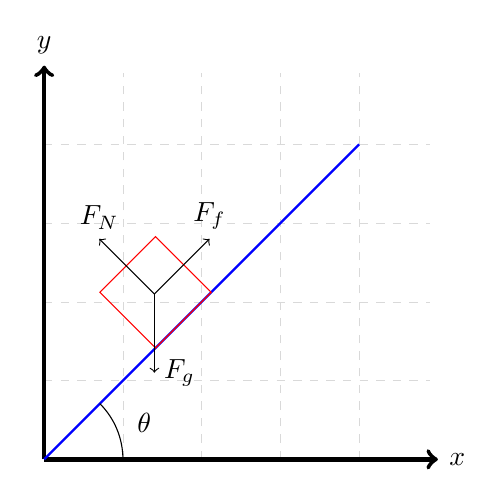
\begin{tikzpicture}
\draw[help lines, color=gray!30, dashed] (0,0) grid (4.9,4.9);
\draw[->,ultra thick] (0,0)--(5,0) node[right]{$x$};
\draw[->,ultra thick] (0,0)--(0,5) node[above]{$y$};
\draw[blue, thick] (0,0) -- (4,4);
\draw (1, 0) arc (0:45:1) node[xshift=10pt, anchor=north west]{$\theta$};
\draw [red, rotate=45, shift={(1, -1)}] (1,1) rectangle (2,2);
\draw[->] (1.4, 2.1) -- (1.4, 1.1) node[anchor=west]{$F_g$};
\draw[->] (1.4, 2.1) -- (2.1, 2.8) node[anchor=south]{$F_f$};
\draw[->] (1.4, 2.1) -- (0.7, 2.8) node[above]{$F_N$};
\end{tikzpicture}
\label{fig: block-ramp}
\end{figure}

We let the static friction force be $\vec{F}_f = f \unit{t}$ where $f$ is the magnitude
of the force of friction and $\unit{t}$ is the direction tangent to the plane, which is
$\unit{t} = \cos \theta \unit{x} + \sin \theta \unit{y}$.

The normal force is $\vec{F}_N = N \unit{n}$ where $\unit{n} = - \sin \theta \unit{x} +
\cos \theta \unit{y}$ is the vector normal to the plane. The normal force resists whatever
is pushing down on the block, so we have $N = mg$. We can now apply Newton's second
law:

\begin{align*}
m \ddot{\vec{r}} &= \sum \vec{F} \\
&= \vec{F}_g + \vec{F}_N + \vec{F}_f \\
&= -mg\unit{y} + mg \left(- \sin \theta \unit{x} + \cos \theta \unit{y} \right) + f \left(
\cos \theta \unit{x} + \sin \theta \unit{y} \right) \\
&= \left( f \cos \theta - mg \sin \theta \right) \unit{x} + \left( f \sin \theta + mg \cos
\theta - mg \right) \unit{y}
\end{align*}

This leads to equations for x and y:

\begin{align*}
&\ddot{x} = \frac{f}{m} \cos \theta - g \sin \theta \\
&\ddot{y} = \frac{f}{m} \sin \theta + g \cos \theta - g
\end{align*}

Provided that $f$, $m$, $\theta$, and $g$ are taken to not depend on time or position,
each of these equations may be integrated to find

\begin{align*}
& x = \left( \frac{f}{m} \cos \theta - g \sin \theta \right) \frac{t^2}{2} + v_{0,x} t
+ x_0 \\
& y = \left( \frac{f}{m} \sin \theta + g \left[ 1 - \cos \theta \right] \right) \frac{t^2}{2}
+ v_{0,y} t + y_0
\end{align*}

where the initial conditions are $v_{0,x} = \dot{x}(0)$, $x_0 = x(0)$, $v_{0,y} =
\dot{y}(0)$, and $y_0 = y(0)$.

\textbf{Extension:} How does this solution change if we take one of the constants to not be constant, but
dependent on either position or time?


\section{Foucalt Pendulum}

\chapter{References}

\bibliographystyle{unsrt}
\bibliography{main}
\end{appendices}

\end{document}